
\section{Research Process}
Part of any research process is rigorous record keeping to ensure experiments can be independently and reliably reproduced.
While researchers keep meticulous journals, when dealing with software this bookkeeping can be largely automated.


\subsection{Version Control}
Software engineering primarily relies on version control systems, such as GitHub, to keep track of code changes.

....

\subsection{Experiment Tracking}
\begin{figure}[h]
    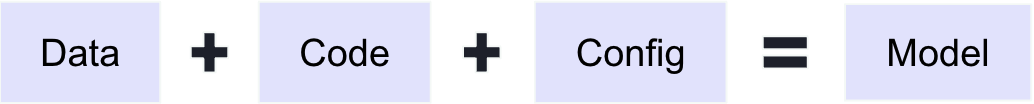
\includegraphics[width=\linewidth]{chapters/NLP/figures/model.png}
    \label{fig:model}
\end{figure}
An experiment is defined by the training code, data, and a configuration file.
When ML and Data Science are involved, the data generating process has to be documented.
In software engineering we say that code doesn't exist until it is "checked into" version control.
Similarly, data doesn't exist until it is stored in the cloud.
In addition to the raw data, we should also store documentation about how it was obtained, by whom, when, and if there have been any additional processing steps.
This should be done in a way that is easy to replicate and understand -- ideally it is documented in code as well.

While version control system are specialized to keep track changes in plain text files, they are not well suited for tracking changes in larger file objects.
To keep track of data (and model) versions the ML community has developed specialized tools\footnote{Weights\&Biases, Neptune}, which we have integrated into Sheepy.
As part of the training run a new experiment is initialized and all hyperparameters are tracked, along with the versions of all dependencies

In addition, these tools allow visualization of metrics, plots, comparison to previous experiments, as well as enables collaboration and sharing of results by directly linking to the tracked experiments.
While being able to repeat previous experiments is important, it is even better if we don't have to -- ML experiments can be expensive.
In addition it is useful to generate formally track \textit{artifacts}, where an artifact refers to a file that is not a code file, but is an important piece of data that is used to generate the results or is the result of an experiment, such as datasets and models.
The file itself is uploaded to a cloud storage service\footnote{Amazon S3, Google Cloud Storage}, and we store a reference to the file as part of the experiment.
Additionally we can store metadata, such as how many samples the data contains, the size and type of fields, when it was created etc..
This facilitates discovery, analysis, iteration, and collaboration.


\subsection{Data Preparation}
One should ensure that all steps necessary to obtain and pre-process the data are documented, ideally in code.
To this end, we provide utilities to handle
\begin{itemize}
    \item Data download
    \item Pre-processing
    \item Splitting into training, validation, and test sets
    \item Feeding data to the model during training
\end{itemize}

We'll go over each of these steps in more detail in the next sections.
The goal is to rerun an experiment from scratch with a single command and we build on top of PyTorch Lightning's \pythoninline{DataModule} class to handle these steps.
\subsubsection{Data Download}
Downloading the dataset from cloud storage and caching are handled in the \pythoninline{prepare_data} method and only executed once per run.
We will first check if the data is already cached, and if not, download it.

\subsubsection{Data Preprocessing}
In general, pre-processing refers to transformation steps we want to apply to the raw data to make it suitable to input into the model.
In NLP, raw text needs to be translated into arrays of integers that the model can map to embedding vectors (see Section \ref{vocabularies_and_words}) (Fig. \ref{fig:tokenization}).
\begin{figure}
    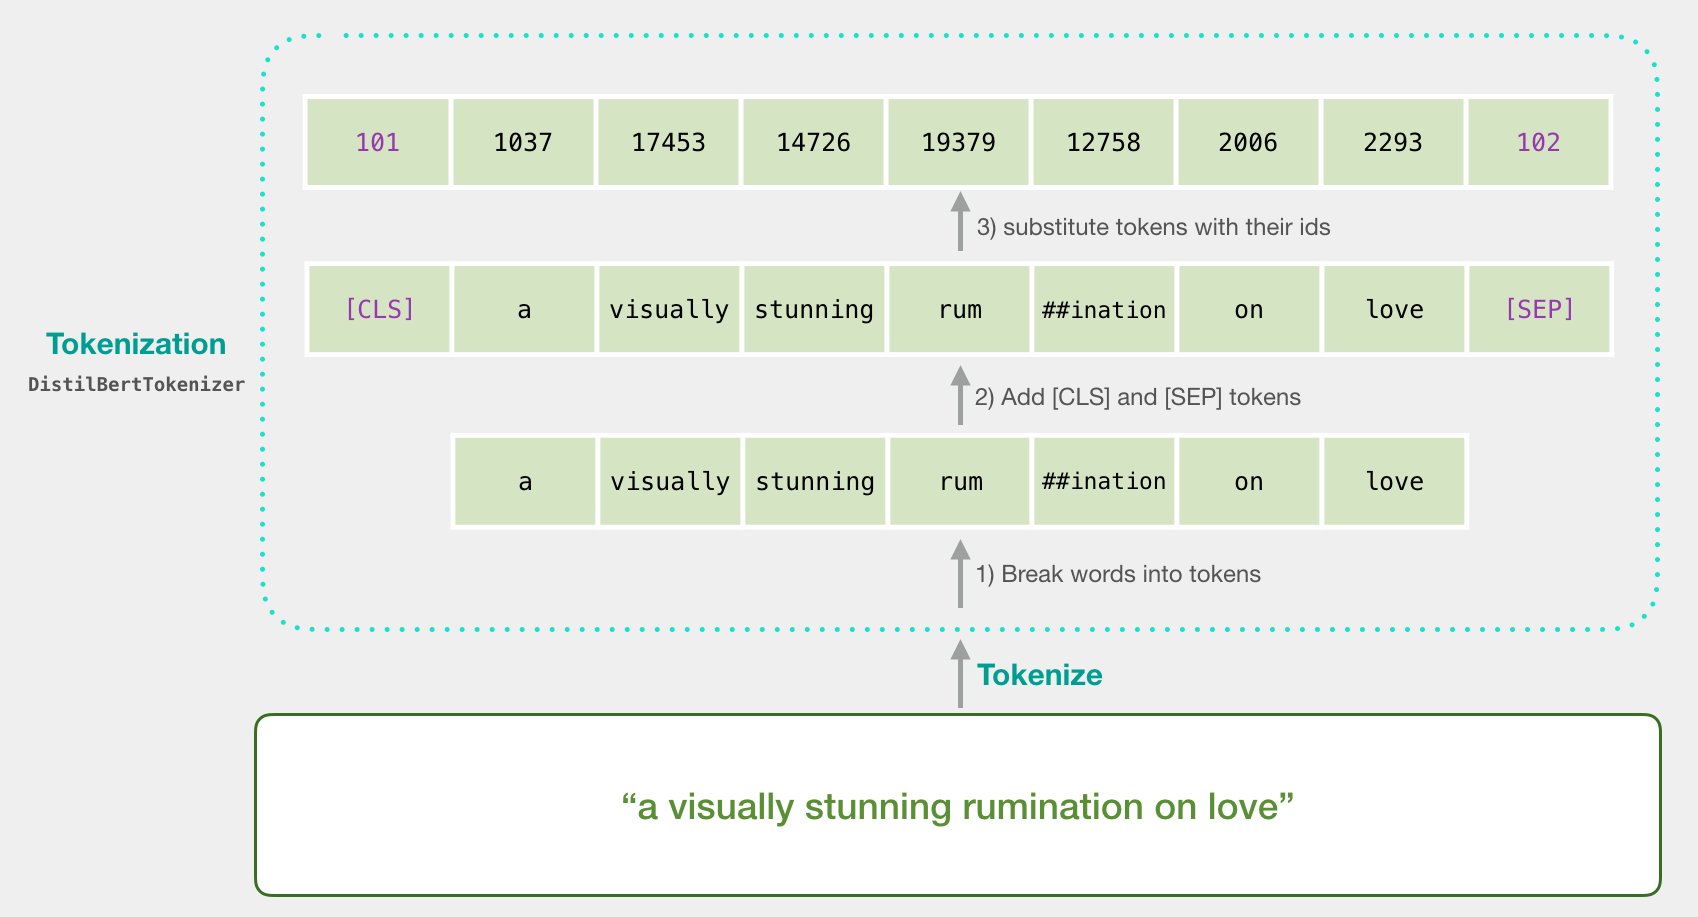
\includegraphics[width=\linewidth]{chapters/NLP/figures/tokenization.png}
    \caption{Tokenization}
    \label{fig:tokenization}
\end{figure}
These steps can be slow and in principle we need to do them only once per sample and cache the results.

\subsubsection{Data Splitting}
\begin{figure}[h]
    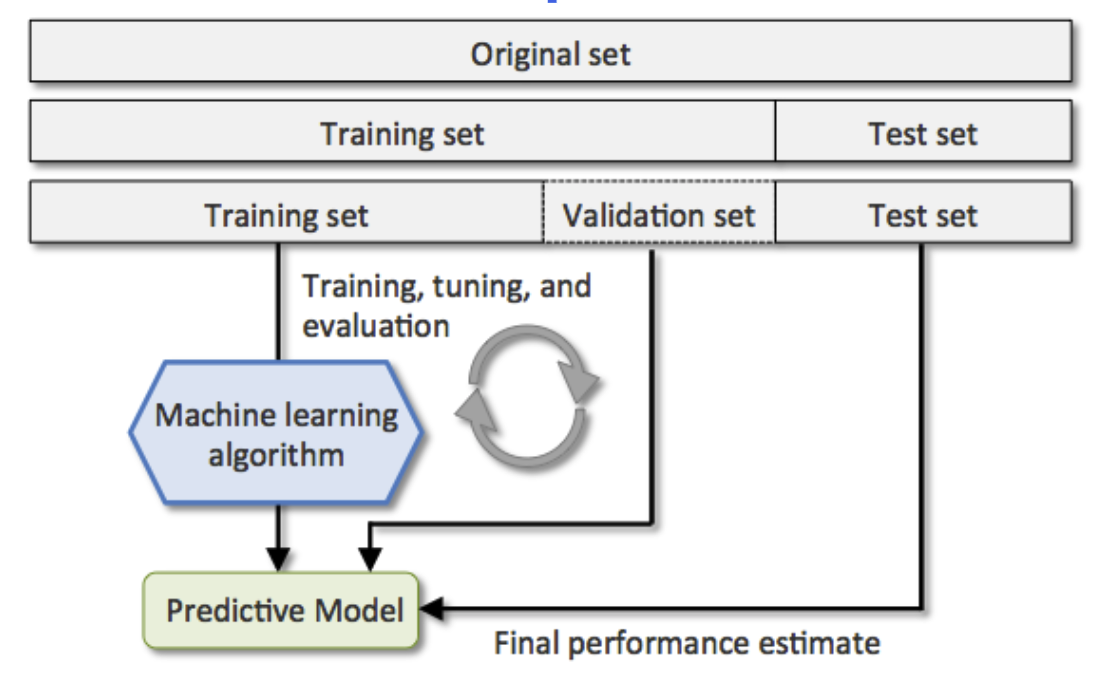
\includegraphics[width=\linewidth]{chapters/NLP/figures/data_splitting.png}
    \caption{Data Splitting}
    \label{fig:data_splitting}
\end{figure}
In order to evaluate the generalization performance of a model it must be tested on data it hasn't seen during training.
The dataset is therefore split into training and validation sets, typically at random (Fig. \ref{fig:data_splitting}).
It should be ensured the randomness is deterministic to reproduce results exactly, which can be achieved by setting a "seed" for the random number generator.
The validation set is used during training to monitor progress and tune hyperparameters.
In addition, it is good practice to hold out another portion of the data, the test set, which is never used during training, but only to report final results.
We otherwise run the risk of tuning hyperparameters to the validation data, thereby overestimating real performance.
Cross validation?
\subsubsection{Feeding Data to the Model}
\begin{figure}[h]
    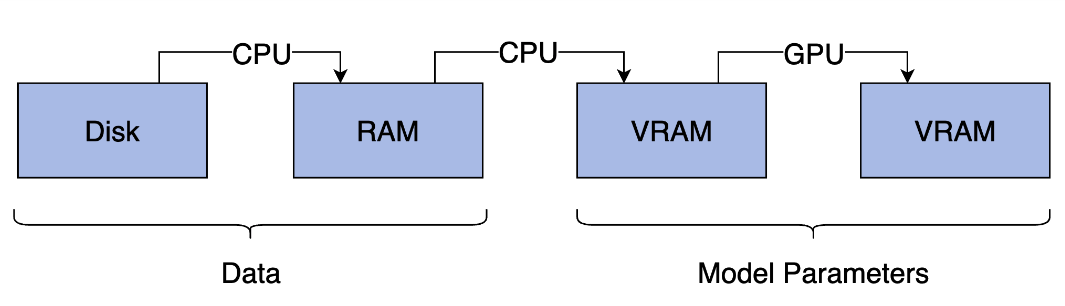
\includegraphics[width=\linewidth]{chapters/NLP/figures/ram_cpu_vram.png}
    \caption{Data needs to be moved from disk to RAM to VRAM so that it can be used to update the model parameters.}
    \label{fig:ram_cpu_vram}
\end{figure}
Model parameters are stored in GPU memory (known as VRAM); in order to update them, the GPU needs to process data from the training set.
After downloading the data from cloud storage it resides on local disk, from where it needs to be moved to RAM and finally VRAM.
Loading data into the model needs to be fast, or we run the risk of starving the GPU, meaning the GPU processes each batch of data faster than the CPU can deliver the next one, leading to low resource utilization and slow training.
We use PyTorch's \pythoninline{DataLoader} class to parallelize this process across multiple CPU workers.
A \pythoninline{DataLoader} takes as argument a \pythoninline{Dataset} and provides a stream of batches of data.
The \textit{batch size} is an important parameter that needs to be tuned on a case by case basis, as we will explain in the next section.

\subsection{Training}
\begin{figure}[h]
    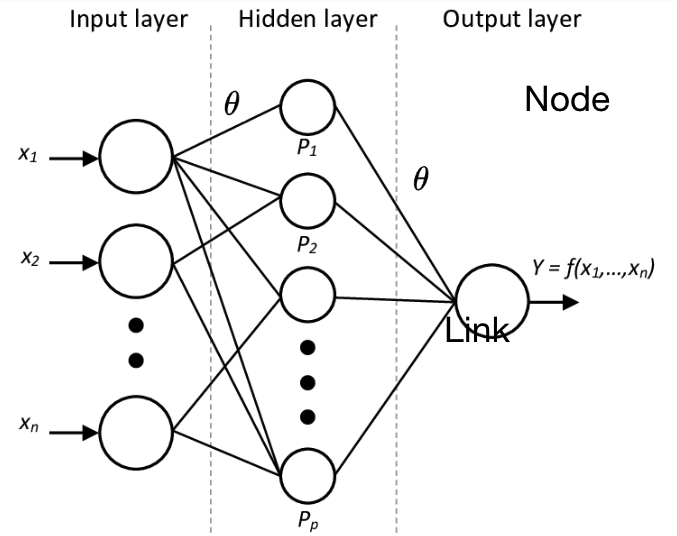
\includegraphics[width=\linewidth]{chapters/NLP/figures/model_architecture.png}
    \caption{Deep neural network architecture}
    \label{fig:model_architecture}
\end{figure}

While glossing over some details, model training can summarized in the following steps:
\begin{itemize}
    \item Given data pairs $(x_i, y_i)$, where $x_i$ is an input sample, and $y_i$ is the desired output
    \item Determine a function $f$, such that $f(\theta, x_i) = \hat{y}_i \approx y_i$, where $\theta$ are model parameters and $f$ is the model architecture
    \item Define a loss function $L(\theta) = \sum_i L(\hat{y}_i, y_i)$ that measures how close the model's output is to the desired output
    \item Optimize $\theta$ to minimize $L(\theta)$
\end{itemize}
\begin{figure}[h]
    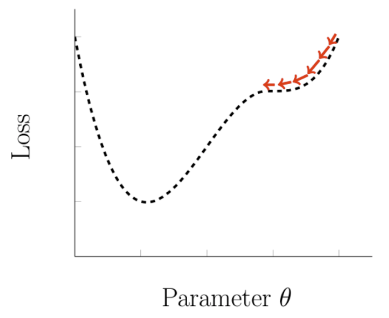
\includegraphics[width=\linewidth]{chapters/NLP/figures/loss.png}
    \caption{Minimizing the loss function}
    \label{fig:loss}
\end{figure}
Here the loss function can take on many forms, depending on the training task, we summarize some of the most common ones in Table \ref{table:losses}.
\begin{table}
    \centering
    \renewcommand{\arraystretch}{1.3}
    \begin{tabular}{|c| c| c|}
    name & function & use \\[0.5ex] \hline
    Mean Squared Error & $\begin{array} {lcl} \frac{1}{N} \sum_{i=1}^N|\hat{y}_i - y_i|^2\end{array}$  & regression \\ [0.5ex]
    Binary Cross Entropy & $\begin{array} {r@{}l@{}} -\frac{1}{N} \sum_{i=1}^N (y_i \cdot log(\hat{y}_i) + (1 - y_i) \cdot log(1-\hat{y}_i)) \end{array}$ & binary classification \\ [0.5ex]
    Cross Entropy & $\begin{array} {r@{}l@{}} -\frac{1}{N} \sum_{i=1}^N y_i \cdot log(\hat{y}_i) \end{array}$ & multiclass classification \\ [0.5ex]
    \end{tabular}
    \caption{Loss functions}
    \label{table:losses}
\end{table}
Parameters in the last layer are then optimized according to the rule
\begin{equation}
    \label{eq:optimization}
    \theta \rightarrow \theta - \alpha \frac{\partial L}{\partial \theta}
\end{equation}
where $\alpha$ is called the \textit{learning rate} and determines the step size, the partial derivative of the loss function with respect to the parameters is called the \textit{gradient}.
For other parameters the rule is similar, but involves the application of the chain rule from calculus.
The algorithm is called \textit{gradient descent} and is the workhorse of all modern deep learning.
In contemporary architectures there are millions to hundreds of billions of parameters, and updating them efficiently is crucial.

To optimize the parameters as outlined in Eq. \ref{eq:optimization} we need to evaluate the gradient of the loss function given the data $(x_i, y_i)$.
To compute the optimial update step we need to sum over all samples in the dataset, compute and store all the gradients, update the parameters once, and repeat the process until convergence.
This however is not practical, given the size of typical datasets and the number of model parameters -- each step would be very computationally expensive and the training slow.

On the other end of the spectrum we could use only a single sample to compute approximations of the optimal gradients, and they will take us close to the global minimum.
This method is called \textit{stochastic gradient descent} and generally works well, but it comes with some tradeoffs:
\begin{itemize}
    \item Loading single samples from the dataset is slow, due to CPU, RAM and bus overhead when copying data to VRAM
    \item There is overhead in the GPU related to scheduling of compute operations
    \item The gradients are much more noisy than the optimal ones, and the model will learn more slowly (see Fig. \ref{fig:mini-batch})
\end{itemize}
There is a happy middle ground called \textit{mini-batch gradient descent} which is a combination of stochastic gradient descent with mini-batches.
Using mini-batches allows for a more accurate estimate of the gradient, and reduces the overhead per sample, as we can take advantage of hardware accelerated vectorized compute operations in CPUs and GPUs.
In practice, we will choose a batch size that is much smaller than the number of samples in the dataset, and as big as possible without running out of VRAM, where the latter condition is typically the more relevant constraint.

\begin{figure}[h]
    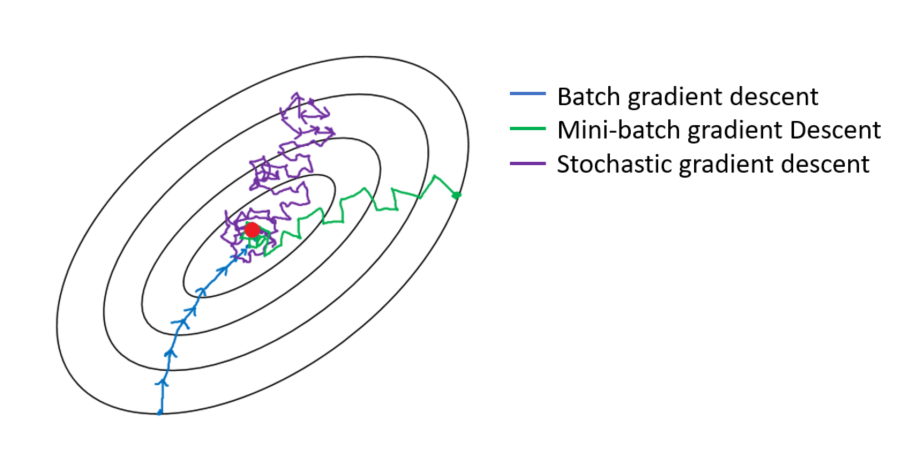
\includegraphics[width=\linewidth]{chapters/NLP/figures/mini-batch.png}
    \caption{Batch vs mini-batch vs stochastic gradient descent}
    \label{fig:mini-batch}
\end{figure}

\subsection{Metrics and Sanity Checking}
\label{metrics_and_sanity_checking}
Here we discuss metrics used to evaluate the performance of classification models.
While
We automatically generate metrics and plots relevant for text classification projects.
